\documentclass{article}

\usepackage{authblk}
\usepackage{hyperref}
\usepackage{float}
\usepackage{multirow}
\usepackage{graphicx}
\usepackage{subcaption}
\usepackage{booktabs}
\usepackage{amsmath}  % Add the amsmath package
\hypersetup{
    colorlinks=true,
    linkcolor=blue,
    filecolor=magenta,      
    urlcolor=cyan,
}
\providecommand{\keywords}[1]{\small \textbf{Keywords:} #1}

\title{Macro Attention Indices for Stock Return Predictability}
\author{Aaron Arauz Baumender (22-748-388) 
\\ Michael Adrian Geiser Pasquel (22-738-645)
\\ Andreas Stavropoulos (22-739-965)
\\ Zhiyi Tang (21-746-763)}
\affil{University of Zurich}
\date{December 2023}

\begin{document}

\maketitle

\begin{abstract} 
\noindent We conduct forecasts for equity risk premia utilizing Ridge regression and neural network models trained on sets of macroeconomic factors and macroeconomic attention indices. The macroeconomic factors set comprises the 14 features recommended in previous works by Goyal and Welch (2008). The set of macro attention indices includes the eight features constructed by Fisher et al. (2022). Equity risk premia represent the annualized excess return of the one-month S\&P 500 index over the prevailing risk-free rate, approximated by the yield on short-term Treasury Bills. Our analysis focuses on the period between 1985 and 2018, given the availability of the data. However, our results deviate from previous research, suggesting the need for further investigation into the datasets.
\end{abstract}

\hfill

\noindent \keywords{Equity risk premia; Macroeconomic factors; Macro economic attention indices; Neural networks; Financial forecast}\\

\newpage

\tableofcontents

\newpage

\section{Introduction}

Equity risk premia, representing the excess return investors expect to receive for holding equities over a risk-free asset, are integral to investment decision-making. The challenge of accurately forecasting these premia has prompted researchers to explore diverse factors, ranging from traditional macroeconomic indicators to emerging metrics like macro attention indices. This study aims to contribute to the predictive modeling landscape by investigating the forecasting capacity of equity risk premia using both Ridge regression and neural network models, trained independently with distinct sets of macroeconomic factors and macro attention indices.

\subsection{Background}

Traditional approaches to forecasting equity risk premia have primarily focused on macroeconomic factors such as interest rates, inflation, and economic growth. Concurrently, the burgeoning field of behavioral finance has introduced macro attention indices—quantifiable measures capturing the collective attention of market participants. These indices reflect the market's sensitivity to information flows and the evolving sentiment among investors.

The rationale for this study lies in recognizing the pivotal interplay between macroeconomic factors and macro attention indices in understanding and predicting equity risk premia. By employing two distinct modeling approaches—Ridge regression models and neural networks—we seek to disentangle the unique contributions of each set of variables, providing a nuanced understanding of their individual and collective impact on forecasting performance.

\subsection{Objectives}

This research has the following key objectives:
\begin{itemize}
  \item Assess the individual predictive capacity of macroeconomic factors in forecasting equity risk premia using Ridge regression and neural network models.
  \item Evaluate the effectiveness of macro attention indices in predicting equity risk premia through both Ridge and neural network models.
\end{itemize}

\subsection{Significance of the Study}

The significance of this study extends beyond traditional forecasting methodologies. By employing both Ridge and neural network models, and considering two distinct sets of variables, we aim to provide a comprehensive analysis that can inform investors, policymakers, and researchers. The findings will contribute insights into the relative strengths and weaknesses of different modeling approaches, ultimately enhancing the understanding of equity market dynamics.

In the subsequent sections, we will delve into a detailed literature review, establish a robust theoretical framework, and conduct empirical analyses to unravel the intricate relationships between macroeconomic factors, macro attention indices, and the forecasting of equity risk premia.

\section{Literature Review}

The literature on forecasting equity risk premia spans studies exploring various factors and methodologies. In this section, we review key contributions related to macroeconomic factors, macro attention indices, and their intersection in predicting equity risk premia.

\subsection{Macroeconomic Factors and Equity Risk Premia}

Historically, research emphasized the role of macroeconomic variables in forecasting equity risk premia. Studies by Fama and French (1988) and Goyal and Welch (2003) explored the impact of dividends and book value on equity markets, providing foundational insights into the relationships between traditional macroeconomic indicators and risk pricing.

Recent contributions by Lo and Singh (2003) and Gu et al. (2019) extended this research, employing advanced econometric techniques to analyze non-Ridge relationships between macroeconomic factors and risk premia. Their findings suggest intricate dynamics between certain macroeconomic variables and risk premia, highlighting the need for sophisticated modeling.

\subsection{Macro Attention Indices and Financial Markets}

The emergence of macro attention indices represents a paradigm shift in understanding how information dissemination influences market dynamics. Studies by Andrei and Hasler (2006) and Nikkien et al. (2006) introduce the concept of macro attention and its role in shaping investor sentiment, capturing collective attention from online and media sources.

Recent research by Ma et al. (2022) shows that incorporating macro attention indices in forecasting models enhances predictive accuracy, especially during heightened market uncertainty. This underscores the importance of considering not only traditional economic indicators but also the broader information environment in forecasting equity risk premia.

\subsection{Comparing Predictive Power of Macroeconomic Factors and Macro Attention Indices}

Previous studies independently explored the impact of macroeconomic factors and macro attention indices on equity risk premia prediction using simple Ridge models. Using a more complex model might provide a more robust framework for predicting market movements. This study addresses this gap by employing Ridge regression models and neural networks to dissect the contributions to forecasting equity risk premia.

Moreover, we delve into specific macroeconomic indicators, such as inflation rates and interest rates, and assess their interplay with macro attention metrics. This comprehensive analysis aims to uncover nuanced relationships that could enhance our understanding of equity risk premia dynamics.

In the following sections, we establish a theoretical framework, outline the methodology, present empirical findings, and discuss the implications of our research for both academic literature and practical applications.

\section{Theoretical Framework}

The theoretical framework guiding this study integrates principles from financial economics, behavioral finance, and the application of machine learning techniques. Our approach to forecasting the S\&P 500 equity risk premia involves a synthesis of traditional economic drivers and contemporary behavioral factors.

\subsection{Market Dynamics Beyond Efficiency}

Contrary to the traditional Efficient Market Hypothesis (EMH), which posits that financial markets rapidly assimilate all available information, our framework acknowledges the existence of market dynamics beyond complete efficiency. We recognize that market anomalies and deviations from efficiency persist, particularly during periods of heightened investor attention. These anomalies challenge the notion of a consistently efficient market and underscore the need for alternative frameworks.

\subsection{Behavioral Finance and Investor Attention}

Incorporating insights from behavioral finance, our framework introduces psychological aspects into financial decision-making. The concept of investor attention emphasizes that market participants may exhibit herd behavior and react to attention-grabbing information, leading to periods of overreaction or underreaction in the market. By integrating macro attention indices in our forecasting models, we account for the role of sentiment and investor attention in shaping market dynamics, acknowledging the limitations of purely rational decision-making assumptions.

\subsection{Neural Networks in Financial Forecasting}

Neural networks provide a flexible framework for capturing complex, non-linear relationships within data. Unlike the traditional Ridge model, which may struggle to capture intricate dynamics, our framework leverages the capabilities of neural networks. Previous studies have demonstrated the effectiveness of neural networks in uncovering patterns that linear models might overlook. By employing neural networks in our analysis, we aim to enhance our ability to model and predict the nuanced interactions between macroeconomic factors and attention-based metrics impacting equity risk premia. This adaptability is particularly valuable in the context of the evolving and dynamic nature of financial markets.

\subsection{Model Specification}

For our study, the equity risk premia (GSPC) will be forecasted using both Ridge regression and neural network models. The macroeconomic factors (MEF) include:

\begin{table}[H]
\centering
\begin{tabular}{|l|l|p{7.5cm}|}
\hline
\textbf{Variable} & \textbf{Name} & \textbf{Description} \\
\hline
dp & Log Dividend-Price & Represents the proportion of dividends paid by S\&P 500 companies relative to the market price. \\
dy & Log Dividend Yield & Signifies the yield on S\&P 500 dividends, indicating the annual dividend income as a percentage of the market price. \\
ep & Log Earnings-Price & Indicates the proportion of earnings generated by S\&P 500 companies relative to the market price. \\
de & Log Dividend-Payout & Reflects the proportion of earnings paid out as dividends by S\&P 500 companies. \\
rvol & Equity Premium Vol & Measures the variability or volatility in the equity premium over a 12-month period, providing insights into market risk. \\
bm & Book-to-Market Ratio & Represents the ratio of the book value of Dow Jones Industrial Average companies to their market value, indicating the value investors assign to a company's assets. \\
ntis & Net Equity Expansion & Quantifies the net expansion or contraction of equity in the market, considering the 12-month sum of net equity issues by NYSE-listed stocks. \\
tbl & Treasury Bill Rate & Represents the interest rate on three-month Treasury bills in the secondary market, serving as a benchmark for short-term risk-free rates. \\
lty & Long-Term Yield & Signifies the yield on long-term government bonds, reflecting the return on long-term fixed-income securities. \\
ltr & Long-Term Return & Represents the historical return on long-term government bonds, providing insights into past performance. \\
tms & Term Spread & Represents the difference between the long-term yield and the treasury bill rate, offering insights into the slope of the yield curve. \\
dfy & Default Yield Spread & Signifies the spread between Moody's BAA corporate bond yield and Moody's AAA corporate bond yield, indicating the additional yield demanded for lower-rated corporate bonds. \\
dfr & Default Return Spread & Represents the spread between the long-term corporate bond return and the long-term government bond return, reflecting the additional return required for investing in corporate bonds with default risk. \\
infl & Inflation & Calculated from the Consumer Price Index for all urban consumers, using two periods of lagged inflation, reflecting the rate of change in the general price level of goods and services over time. \\
\hline
\end{tabular}
\caption{Macroeconomic Factors (MEF) for Equity Risk Premia Forecasting.}
\label{tab:MEF}
\end{table}

The macro attention indices (MAI) include:

\begin{table}[H]
\centering
\begin{tabular}{|l|l|p{7.5cm}|}
\hline
\textbf{Variable} & \textbf{Name} & \textbf{Description} \\
\hline
credit\_rating & Credit Rating & Reflects entities' creditworthiness, influencing investor risk perceptions; a higher credit rating indicates lower default risk. \\
gdp & Gross Domestic Product & Represents total goods and services value within a country, a key indicator of economic health. \\
house\_mkt & House Market & Captures housing market trends, providing insights into broader economic conditions. \\
inflation & Inflation & Measures the percentage change in the general price level, influencing purchasing power and monetary policy. \\
monetary & Monetary & Encompasses attention on monetary policy, including interest rates and central bank decisions. \\
oil & Oil & Reflects attention on the oil market, crucial for understanding energy-related economic trends. \\
unemp & Unemployment Rate & Captures attention related to employment trends and economic stability. \\
usd & US Dollar & Reflects attention on the U.S. dollar, impacting international trade and economic conditions. \\
\hline
\end{tabular}
\caption{Macro Attention Indices (MAI) for Equity Risk Premia Forecasting.}
\label{tab:MAI}
\end{table}

The S\&P 500 (GSPC) equity risk premia include:
\begin{table}[H]
\centering
\begin{tabular}{|l|l|p{7.5cm}|}
\hline
\textbf{Variable} & \textbf{Name} & \textbf{Description} \\
\hline
GSPCprem & Equity Risk Premia  & Reflects the excess return an investor expects to receive from holding equities (stocks) compared to a risk-free (government bonds). \\
\hline
\end{tabular}
\caption{S\&P 500 (GSPC) Equity Risk Premia.}
\label{tab:GSPC}
\end{table}

These variables form the basis for our models, allowing us to independently assess the predictive capabilities of Ridge regression and neural network models. In the subsequent section, we detail the methodology employed for model implementation and evaluation.

\section{Methodology}

Forecasting GSPC equity risk premia involves the application of both Ridge regression and neural network models using the identified MEF and MAI data. The aim is to independently assess the predictive capabilities of these models and understand how the inclusion of behavioral and attention-based metrics enhances forecasting accuracy.

\subsection{Data Management}

The historical data is collected over a time period of 34 years (1985 to 2018) and with three different frequencies (daily, monthly, quarterly). The datasets are organized to align with the time series nature of financial and economic variables, ensuring chronological order for proper model training and evaluation.

\subsubsection{Data Collection (raw data)}
  
MEF monthly and quarterly raw data is collected from powder197/Goyal-and-Welch-2008- Github repository. This raw data contains the following information: "date", "index", "lag\_index\_1", "d12", "e12", "bm", "tbl", "aaa", "baa", "lty", "ntis", "infl", "ltr", "corpr", and "svar". This information is used in a later stage to construct the 14 macroeconomic factors.

MEF daily raw data is implied from MEF monthly raw data. More specifically, daily "infl", "ltr", and "corpr" variables are implied from monthly data as follows: $\text{ddp} = (1+\text{mdp})^{1/\text{ndm}}-1$, were $\text{ddp}$ stands for daily data point, $\text{mdp}$ stands for monthly data point, and $\text{ndm}$ means number of days in month. 
Daily "d12", "e12", "bm", "tbl", "aaa", "baa", "lty", and "ntis" variables are computed as linear interpolations between monthly data points. Lastly, daily "svar" varialbe is simply calculated as $(\text{mdp}/\text{ndm})$, i.e. prorated data through the month.

MAI daily and monthly raw data is collected from charlesmartineau/mai\_rfs Github repository. This raw data contains the following information: "date", "credit\_rating\_ni", "gdp\_ni", "house\_mkt\_ni", "inflation\_ni", "monetary\_ni", "oil\_ni", "unemp\_ni", "usd\_ni", "credit\_rating\_wi", "gdp\_wi", "house\_mkt\_wi", "inflation\_wi", "monetary\_wi", "oil\_wi", "unemp\_wi", and "usd\_wi". Columns ending with "\_ni" and "\_wi" correspond to information provided by the New York Times and Wall Street Journal, respectively. This information is used in a later stage to construct the eight macro attention indexes.

MAI quarterly raw data is implied from MAI monthly raw data.

GSPC daily, monthly, and quarterly raw data is collected from Yahoo Finance. This raw data contains the following information: "date", "GSPC"	"lead\_GSPC\_1M", "rfr", "lead\_date". This information is used in a later stage to construct the equity risk premia.

\subsubsection{Data Cleaning (interim data)}

The collected data undergoes preprocessing steps to improve the quality and compatibility of the input features. This process specifically addresses missing values in the MAI raw databases.

To illustrate the calculation of MAI daily, monthly, and quarterly interim data, let's consider the "credit\_rating" variable as an example. If "credit\_rating\_ni" is $0$ while "credit\_rating\_wi is not $0$, the $0$ value of "credit\_rating\_ni" is replaced with the value of "credit\_rating\_wi". Conversely, if "credit\_rating\_wi" is $0$ but "credit\_rating\_ni" is not $0$, the $0$ value of "credit\_rating\_wi" is replaced with the value of "credit\_rating\_ni". In the case where both "credit\_rating\_ni" and "credit\_rating\_wi" are $0$, we retain the previous values of both variables, respectively. This approach is rooted in the rationale that if one journal (but not both) fails to produce the "credit\_rating" index, it indicates that no relevant news related to credit rating was published in that specific journal. In such instances, the other magazine contains updated information embedded in the index. However, when both journals fail to produce the "credit\_rating" index, it suggests that no change in credit rating information was released. Consequently, we can safely assume that the previous information remains unchanged, reflecting a status quo in the index.

MEF raw requires no interim treatment. GSPC raw data requires dropping some features which will not be used, namely "lag\_GSPC\_1", "lead\_GSPC\_2", "lag\_rfr\_1", "lag\_date\_1", "lead\_date\_2". The calculation or equity risk premia will be performed directly at a later stage.

\subsubsection{Data Processing (processed data)}
The preprocessed data is used to construct the data for model training.

MEF processed data consists of "date" and the 14 macroeconomic factors. The calculations are as follows:
\begin{equation*}
    \text{dp} = \log{(\text{d12})} - \log{(\text{index})},
\end{equation*}
\begin{equation*}
    \text{dy} = \log{(\text{d12})} - \log{(\text{lag\_index\_1})},
\end{equation*}
\begin{equation*}
    \text{ep} = \log{(\text{e12})} - \log{(\text{index})},
\end{equation*}
\begin{equation*}
    \text{de} = \log{(\text{d12})} - \log{(\text{e12})},
\end{equation*}
\begin{equation*}
    \text{tms} = \text{lty} - \text{tbl},
\end{equation*}
\begin{equation*}
    \text{dfy} = \text{baa} - \text{aaa},
\end{equation*}
\begin{equation*}
    \text{dfr} = \text{corp} - \text{ltr}.
\end{equation*}
All other factors, namely rvol, bm, ntis, tbl, lty, and ltr, are directly found from the corresponding columns in the interim data.

MAI processed data consists of "date" and the eight macro attention indexes. The calculation of the index consists of a simple average between the corresponding columns ending with "\_ni" and "\_wi". As an example, "credit\_rating" is computed as follows:
\begin{equation*}
    \text{credit\_rating} = \frac{\text{credit\_rating\_ni}+\text{credit\_rating\_wi}}{2}.
\end{equation*}

GSPC processed data consists of "date" and "GSPCprem" columns. The latter is constructed from interim data as follows:
\begin{equation*}
    \text{GSPCprem} = \big( \frac{\text{lead\_GSPC\_1}}{\text{GSPC}}-1 \big) \times 12 \times 100 - \text{rfr}.
\end{equation*}

For daily data, lead\_GSPC\_1 corresponds to the realization of GSPC 22 days in the future, approximately one month ahead. For monthly data, lead\_GSPC\_1 corresponds to the realization of GSPC one month in the future.

The next tables summarize key statistics of the processed data sets:

\newpage

MEF daily processed data

\begin{tabular}{lrrrrrrr}
\toprule
{} &    dp &    dy &    ep &    de &  rvol &    bm &  ntis \\
\midrule
count &  8503 &  8503 &  8503 &  8503 &  8503 &  8503 &  8503 \\
mean  &    -3.84 &    -3.84 &    -3.05 &    -0.79 &     0.00 &     0.32 &     0.00 \\
std   &     0.32 &     0.32 &     0.37 &     0.38 &     0.00 &     0.11 &     0.00 \\
min   &    -4.53 &    -4.53 &    -4.87 &    -1.24 &     0.00 &     0.12 &    -0.00 \\
25\%   &    -4.04 &    -4.04 &    -3.18 &    -1.02 &     0.00 &     0.24 &    -0.00 \\
50\%   &    -3.90 &    -3.90 &    -2.99 &    -0.86 &     0.00 &     0.31 &     0.00 \\
75\%   &    -3.56 &    -3.56 &    -2.82 &    -0.61 &     0.00 &     0.38 &     0.00 \\
max   &    -3.14 &    -3.14 &    -2.37 &     1.38 &     0.07 &     0.73 &     0.00 \\
\bottomrule
\end{tabular}

\bigskip

\begin{tabular}{lrrrrrrr}
\toprule
{} &   tbl &   lty &   ltr &   tms &   dfy &   dfr &  infl \\
\midrule
count &  8503 &  8503 &  8503 &  8503 &  8503 &  8503 &  8503 \\
mean  &     0.03 &     0.06 &     0.00 &     0.02 &     0.01 &     0.00 &     0.00 \\
std   &     0.03 &     0.02 &     0.00 &     0.01 &     0.00 &     0.02 &     0.00 \\
min   &     0.00 &     0.02 &    -0.00 &    -0.00 &     0.01 &    -0.06 &    -0.01 \\
25\%   &     0.01 &     0.04 &    -0.00 &     0.01 &     0.01 &    -0.01 &    -0.00 \\
50\%   &     0.03 &     0.05 &     0.00 &     0.02 &     0.01 &     0.01 &     0.00 \\
75\%   &     0.05 &     0.07 &     0.00 &     0.03 &     0.01 &     0.02 &     0.00 \\
max   &     0.09 &     0.12 &     0.01 &     0.05 &     0.03 &     0.05 &     0.01 \\
\bottomrule
\end{tabular}

\newline

\bigskip
MAI daily processed data

\begin{tabular}{lrrrrrrrr}
\toprule
{} &  credit\_rating &    gdp &  house\_mkt &  inflation &  monetary &   oil &  unemp &   usd \\
\midrule
count &        8503 & 8503 &    8503 &    8503 &   8503 & 8503 & 8503 & 8503 \\
mean  &           1.01 &    1.39 &       1.24 &       2.21 &      2.08 &    2.44 &    1.56 &    1.35 \\
std   &           0.62 &    0.90 &       0.90 &       1.23 &      1.20 &    1.69 &    0.97 &    0.87 \\
min   &           0.32 &    0.33 &       0.32 &       0.32 &      0.33 &    0.33 &    0.32 &    0.32 \\
25\%   &           0.59 &    0.76 &       0.63 &       1.30 &      1.23 &    1.25 &    0.87 &    0.77 \\
50\%   &           0.85 &    1.17 &       0.92 &       1.96 &      1.81 &    1.95 &    1.32 &    1.10 \\
75\%   &           1.25 &    1.74 &       1.53 &       2.80 &      2.63 &    3.16 &    1.98 &    1.72 \\
max   &           9.40 &    8.72 &       8.63 &      10.81 &     12.47 &   13.50 &    9.33 &    8.40 \\
\bottomrule
\end{tabular}

\newpage

\bigskip
MEF monthly processed data

\begin{tabular}{lrrrrrrr}
\toprule
{} &    dp &    dy &    ep &    de &  rvol &    bm &  ntis \\
\midrule
count &  408 &  408 &  408 &  408.00 &  408.00 &  408.00 &  408.00 \\
mean  &   -3.83 &   -3.83 &   -3.05 &   -0.79 &    0.00 &    0.32 &    0.00 \\
std   &    0.32 &    0.32 &    0.37 &    0.38 &    0.01 &    0.12 &    0.02 \\
min   &   -4.52 &   -4.53 &   -4.84 &   -1.24 &    0.00 &    0.12 &   -0.06 \\
25\%   &   -4.04 &   -4.03 &   -3.19 &   -1.02 &    0.00 &    0.25 &   -0.01 \\
50\%   &   -3.89 &   -3.89 &   -2.99 &   -0.87 &    0.00 &    0.31 &    0.01 \\
75\%   &   -3.56 &   -3.55 &   -2.82 &   -0.61 &    0.00 &    0.38 &    0.02 \\
max   &   -3.15 &   -3.09 &   -2.38 &    1.38 &    0.07 &    0.73 &    0.05 \\
\bottomrule
\end{tabular}


\bigskip
\begin{tabular}{lrrrrrrr}
\toprule
{} &   tbl &   lty &   ltr &   tms &   dfy &   dfr &  infl \\
\midrule
count &  408 &  408 &  408 &  408 &  408 &  408 &  408 \\
mean  &    0.03 &    0.06 &    0.01 &    0.02 &    0.01 &   -0.00 &    0.00 \\
std   &    0.03 &    0.02 &    0.03 &    0.01 &    0.00 &    0.02 &    0.00 \\
min   &    0.00 &    0.02 &   -0.11 &   -0.00 &    0.01 &   -0.10 &   -0.02 \\
25\%   &    0.01 &    0.04 &   -0.01 &    0.01 &    0.01 &   -0.01 &    0.00 \\
50\%   &    0.03 &    0.05 &    0.01 &    0.02 &    0.01 &    0.00 &    0.00 \\
75\%   &    0.05 &    0.07 &    0.03 &    0.03 &    0.01 &    0.01 &    0.00 \\
max   &    0.09 &    0.12 &    0.14 &    0.05 &    0.03 &    0.07 &    0.01 \\
\bottomrule
\end{tabular}

\newline


\bigskip
MAI monthly processed data

\begin{tabular}{lrrrrrrrr}
\toprule
{} &  credit\_rating &   gdp &  house\_mkt &  inflation &  monetary &   oil &  unemp &   usd \\
\midrule
count &           408 & 408 &     408 &     408 &    408 & 408 & 408 & 408 \\
mean  &             1.01 &   1.58 &       1.26 &       2.19 &      2.05 &   2.49 &   1.69 &   1.43 \\
std   &             0.61 &   0.98 &       0.95 &       1.11 &      1.16 &   1.81 &   0.96 &   0.93 \\
min   &             0.36 &   0.33 &       0.38 &       0.41 &      0.41 &   0.43 &   0.41 &   0.40 \\
25\%   &             0.60 &   0.84 &       0.63 &       1.36 &      1.20 &   1.21 &   0.98 &   0.79 \\
50\%   &             0.84 &   1.30 &       0.93 &       2.05 &      1.76 &   1.94 &   1.46 &   1.18 \\
75\%   &             1.27 &   2.03 &       1.50 &       2.88 &      2.63 &   3.20 &   2.26 &   1.77 \\
max   &             4.91 &   5.95 &       6.43 &       8.48 &      7.39 &  13.50 &   5.43 &   6.11 \\
\bottomrule
\end{tabular}

\newpage

\subsection{Data Selection}
Utilizing the \href{https://baumender11.shinyapps.io/Alpha/}{interactive Shiny app} facilitates a lucid visualization of the impact of various features and temporal ranges on predictive outcomes. Users are afforded the flexibility to select any subset of the 14 MEF variables, the 8 MAI variables, temporal spans ranging from January 1, 1985, to December 31, 2018, and temporal frequencies at daily, monthly, or quarterly intervals. The MEF model results are denoted by blue lines, the MAI model results by green lines, and the veritable values by the red line.

Here we employ two cases on quarterly data as illustrative examples. With lower frequency, the lines are easier to identify.

\begin{figure}[H]
    \centering 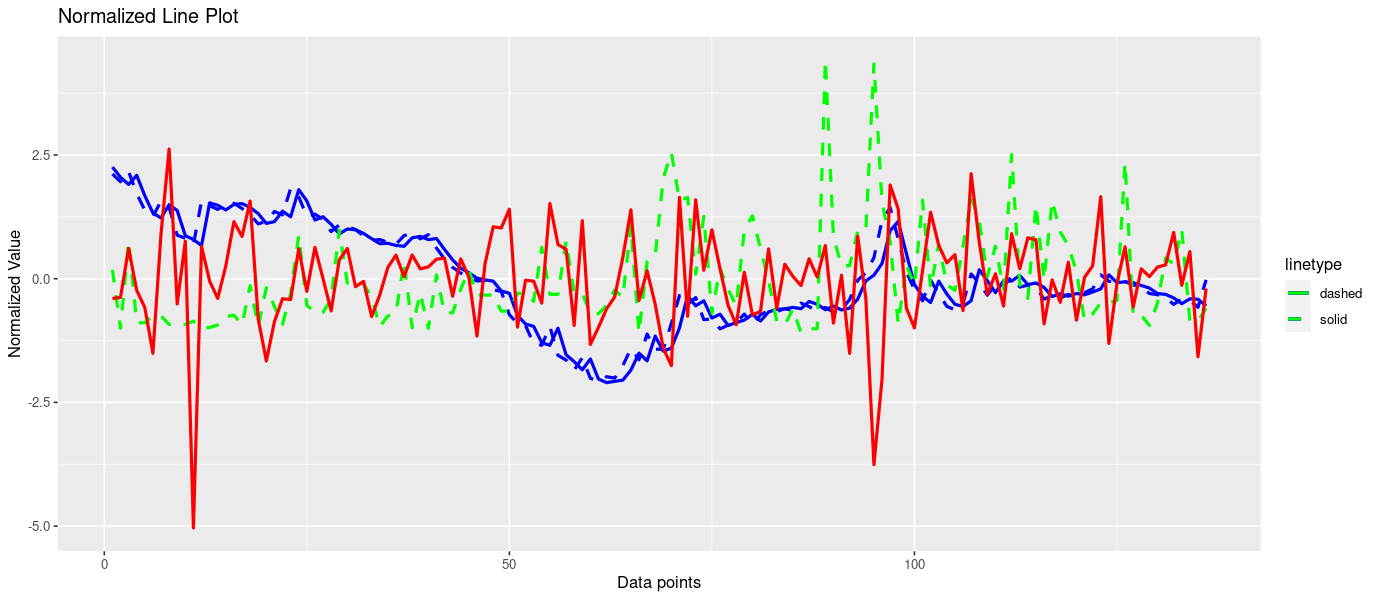
\includegraphics[width=1\linewidth]{MEF_dpdy_MAI_cr.png}
    \caption{Shiny app variable selection outcome, case 1.- \href{https://baumender11.shinyapps.io/Alpha/}{Interactive Shiny App}}
\end{figure}

In the first case, quarterly data between 1.1.1985 and 31.12.2018 of MEF Log Dividend-Price (solid blue), MEF Log Dividend Yield (dashed blue), MAI Credit Rating (dashed green), and MKT GSPC (solid red) are selected.

\begin{figure}[H]
    \centering 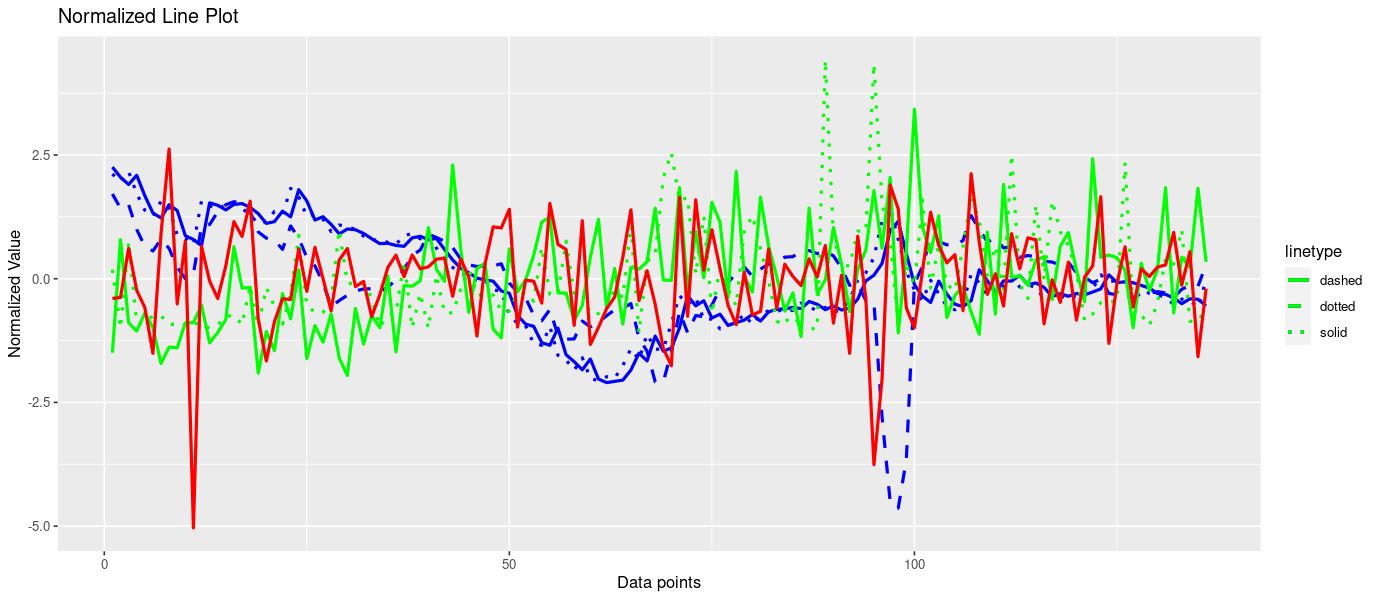
\includegraphics[width=1\linewidth]{MEF_dpdyep_MAI_crgdp.png}
    \caption{Shiny app variable selection outcome, case 2.- \href{https://baumender11.shinyapps.io/Alpha/}{Interactive Shiny App}}
\end{figure}

In the second case, quarterly data between 1.1.1985 and 31.12.2018 of MEF Log Dividend-Price (solid blue), MEF Log Dividend Yield (dotted blue), MEF Log Earnings-Price (dashed blue), MAI Credit Rating (dotted green), MAI Gross Domestic Product (solid green), and MKT GSCP (solid red) are selected.

The \href{https://baumender11.shinyapps.io/Alpha/}{interactive Shiny app} also helps show the correlation heatmaps of the variables chosen in a certain temporal range.

\begin{figure}[H]
  \centering
  \begin{subfigure}{0.3\linewidth}
    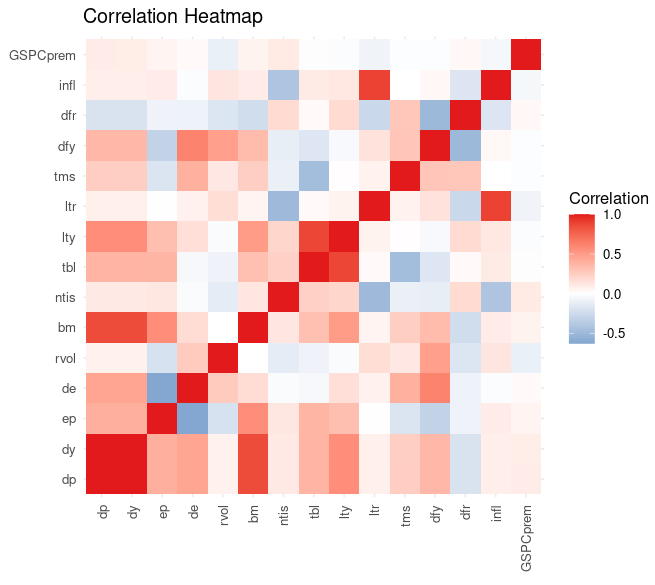
\includegraphics[width=\linewidth]{Cormap_MEF_Daily_85.png}
    \caption{MEF daily.}
  \end{subfigure}
  \hfill
  \begin{subfigure}{0.3\linewidth}
    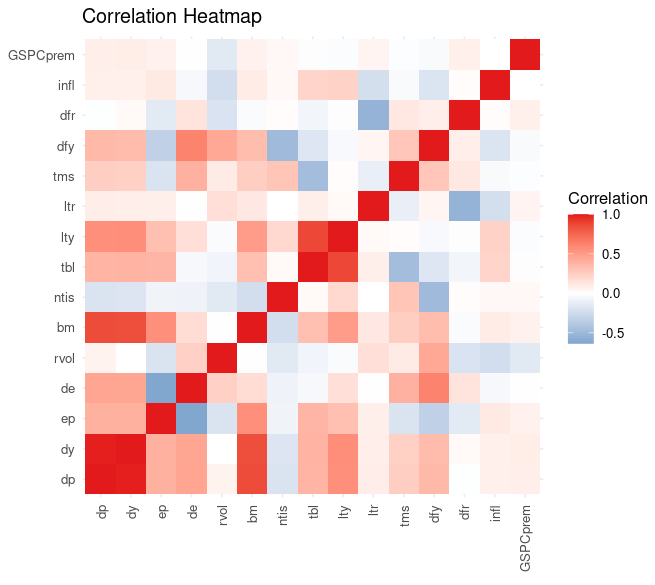
\includegraphics[width=\linewidth]{Cormap_MEF_Monthly_85.png}
    \caption{MEF monthly.}
  \end{subfigure}
  \hfill
  \begin{subfigure}{0.3\linewidth}
    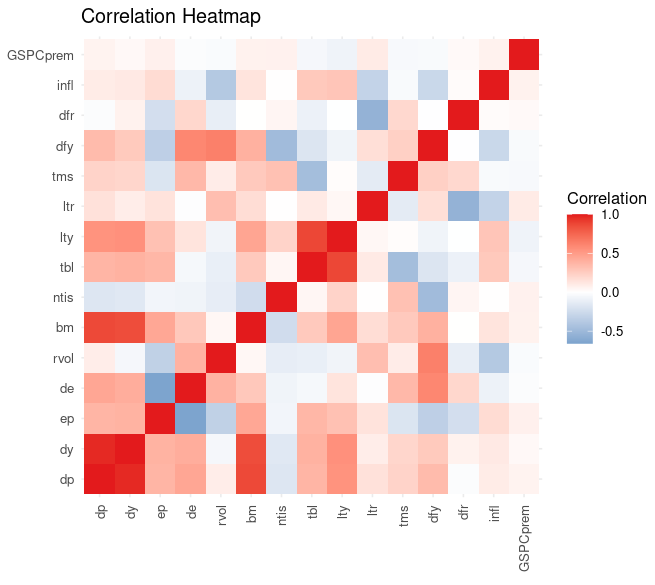
\includegraphics[width=\linewidth]{Cormap_MEF_Quarterly_85.png}
    \caption{MEF quarterly.}
  \end{subfigure}
  \caption{Correlation heatmaps, MEF variables, 1.1.1985 to 31.12.2018}
  \label{fig:cormap1}
\end{figure}

\begin{figure}[H]
  \centering
  \begin{subfigure}{0.3\linewidth}
    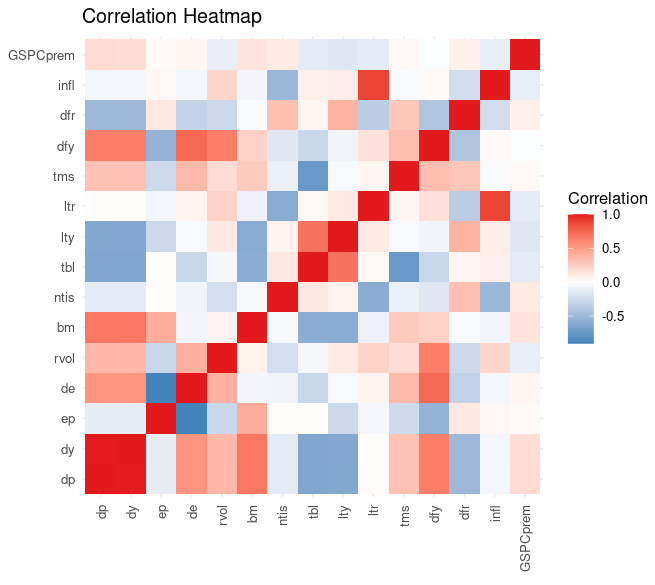
\includegraphics[width=\linewidth]{Cormap_MEF_Daily_00.png}
    \caption{MEF daily.}
  \end{subfigure}
  \hfill
  \begin{subfigure}{0.3\linewidth}
    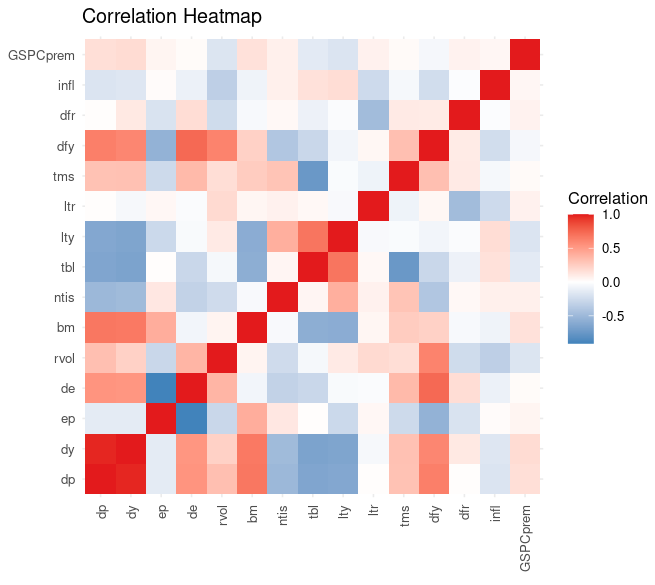
\includegraphics[width=\linewidth]{Cormap_MEF_Monthly_00.png}
    \caption{MEF monthly.}
  \end{subfigure}
  \hfill
  \begin{subfigure}{0.3\linewidth}
    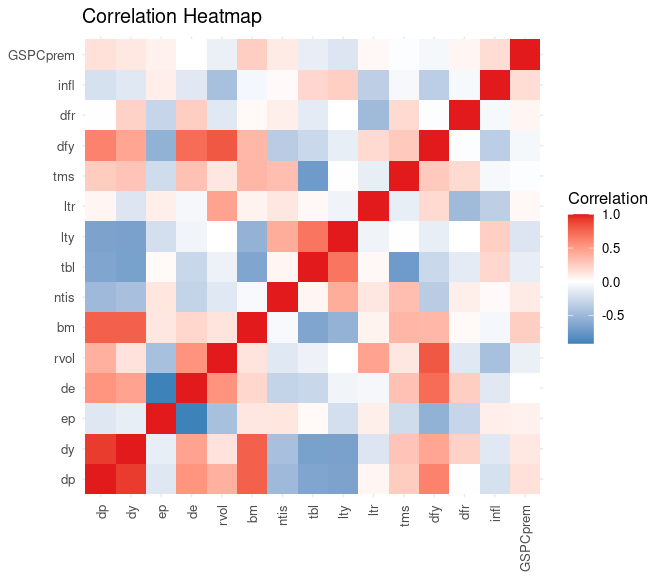
\includegraphics[width=\linewidth]{Cormap_MEF_Quarterly_00.png}
    \caption{MEF quarterly.}
  \end{subfigure}
  \caption{Correlation heatmaps, MEF variables, 1.1.2000 to 31.12.2018}
  \label{fig:cormap2}
\end{figure}

Examining the heatmaps spanning the periods 1.1.1985 to 31.12.2018 (Figure \ref{fig:cormap1}) and 1.1.2000 to 31.12.2018 (FIgure \ref{fig:cormap2}) reveals a discernible shift in the correlation among certain variables, transitioning from positive correlation (indicated by red) to negative correlation (indicated by blue). Nevertheless, when scrutinizing distinct frequencies within the identical temporal span, namely daily, monthly, and quarterly data, negligible disparities are evident in the correlation patterns of the variables.

\subsection{Model Training}

Two distinct approaches are employed for model training: Ridge regression and neural network models. For Ridge regression, the relationship between the GSPC equity risk premia and the MEF/MAI data is modeled using the standard Ridge regression equation. The coefficients are estimated using gradient decent with Ridge regularization to capture the linear relationships between the variables.

For neural network models, a feedforward neural network architecture is employed. The network is designed with input layers corresponding to the MEF/MAI data sets, hidden layers for capturing non-linear relationships, and an output layer for predicting the GSPC equity risk premia. The network is trained using Adam optimizer, learning rate $0.01$, epochs $10$, and batch size $32$, two hidden layers (the first one with $64$ neurons, the second one with $32$ neurons), and dropout layers.

The performance of the models is evaluated using Root Mean Squared Error (RMSE).

\subsection{Comparison and Interpretation}

The results from the Ridge regression and neural network models, expressed in terms of RMSE, are compared to understand their relative strengths and weaknesses in forecasting equity risk premia. Both sets of economic data-MAI and MEF data-are used independently and also combined in order to evaluate the predictive capacity of different combinations. The target variable is the $1$-month GSPC equity risk premia, using as daily and monthly frequency.

\section{Empirical Analysis}

The empirical analysis involves implementing the models specified in the methodology section to forecast the $1$-month GSPC equity risk premia based on the selected macroeconomic factors (MEF) and macro attention indices (MAI). For this, we use daily and monthly data from both sets of economic data.

The findings from the analysis provide insights into the effectiveness of Ridge regression and neural network models in predicting equity risk premia and the impact of attention-based metrics.

\subsection{Data Overview}

In this study, we use six datasets. The table below (Table \ref{tab:Datasets}) shows the characteristics of the datasets.

\begin{table}[H]
\centering
\small
\begin{tabular}{|c|c|c|c|c|}
\hline
Dataset & \begin{tabular}[c]{@{}c@{}}Number of\\ vairiables\end{tabular} & Frequency & Time Period & \begin{tabular}[c]{@{}c@{}}Number of\\ samples\end{tabular} \\ \hline
MEF Daily & 14 & Daily & 1985/01/02-2018/12/31 & 8523 \\ \hline
MAI Daily & 8 & Daily & 1985/01/02-2018/12/31 & 8523 \\ \hline
MKT Daily & 1 & Daily & 1985/01/02-2018/12/31 & 8523 \\ \hline
MEF Monthly & 14 & Monthly & 1985/01/31-2018/12/31 & 408 \\ \hline
MAI Monthly & 8 & Monthly & 1985/01/31-2018/12/31 & 408 \\ \hline
MKT Monthly & 1 & Monthly & 1985/01/31-2018/12/31 & 408 \\ \hline
\end{tabular}
\caption{Description of Datasets used for model training.}
\label{tab:Datasets}
\end{table}

\subsection{Model Implementation}

\subsubsection{Ridge Regression Model}

The ridge regression model is implemented using the MEF and MAI data as independent variables. The model is trained on the four datasets described above (MEF monthly, MAI monthly, MEF daily, MAI daily) to establish the linear relationship with the GSPC data (MKT monthly, MKT daily), the dependent variable. 
\\
For all the datasets we use the following specifications:
\begin{itemize}
    \item K-fold cross-validation with 5 folds to tune the hyperparameter
    \item The grid of tested values is $[10^{-5}, 10^{-4}, 10^{-3}, 10^{-2}, 10^{-1}, 1, 10, 10^{2}, 10^{3}, 10^{4}, 10^{5}]$
    \item The train-test split is $80\%-20\%$.
\end{itemize}

In the case of the monthly datasets, since their size is small (408 points), we train the models 10 times with a different train-test split in each iteration, in order to ensure some robustness. In the end, we report the average RMSE on the test set of the 10 iterations.
\\
\\
In the case of the daily datasets, we train the model only once (for each dataset) and report the RMSE on the test set.

\subsubsection{Neural Network Model}

For the neural network model, we use a feedforward architecture with the following specifications:
\begin{itemize}
    \item Two hidden layers, with 64 and 32 neurons respectively
    \item Two dropout layers following each hidden layer with $30\%$ and $50\%$ dropping rate respectively
    \item Single neuron output
    \item Adam optimiser with learning rate $0.01$
    \item batch size: 32
    \item number of epochs: 10

\end{itemize}
Similarly with the regression model, when working with the monthly data, we train the models 10 times with different train-test splits and report the average RMSE and when we work with the daily data, we only train and predict once. As a side note, we did not expect to extract meaningful results from the monthly datasets, since the amount of data points in them (408) would not be sufficient for efficiently training a neural network. However, we try this approach as a reference and a comparison point with the regression model.

\subsection{Results}

\subsubsection{Performance evaluation}
The results we get from the models described above can be seen in Table 5. For the monthly datasets, the reported RMSE is the average over 10 iterations, as explained before.


\begin{table}[H]
\centering
\begin{tabular}{|c|c|c|}
\hline
\textbf{Model} & \textbf{Input Data} & \textbf{RMSE on Test Set} \\ \hline
\multirow{4}{*}{Ridge Model} & MEF Daily & 53.243 \\ \cline{2-3} 
 & MAI Daily & 54.677 \\ \cline{2-3} 
 & MEF Monthly & 54.307 \\ \cline{2-3} 
 & MAI Monthly & 53.571 \\ \hline
\multirow{4}{*}{NN Model} & MEF Daily & 54.142 \\ \cline{2-3} 
 & MAI Daily & 54.066 \\ \cline{2-3} 
 & MEF Monthly & 52.717 \\ \cline{2-3} 
 & MAI Monthly & 53.096 \\ \hline
\end{tabular}
\caption{Comparison of RMSE of different models.}
\label{tab:RMSE}
\end{table}

\subsubsection{Regression Model Results}
The predictive power of the ridge regression model for all four datasets seems to be non-existent since the RMSE is huge (around 55) relative to the range of the target variable (-250 to 100).\\

If we plot the real values over the predicted ones (at the last iteration for the monthly data), the predictions seem to gather around 0 (with a bit larger oscillation for the daily data). This might indicate the lack of predictive power of the features, leading to the ridge parameter dominating and sending the predictions to small values, regardless of the target. Further discussion of the results and potential interpretations can be found in the next chapter. 

\begin{figure}[h]
    \centering
    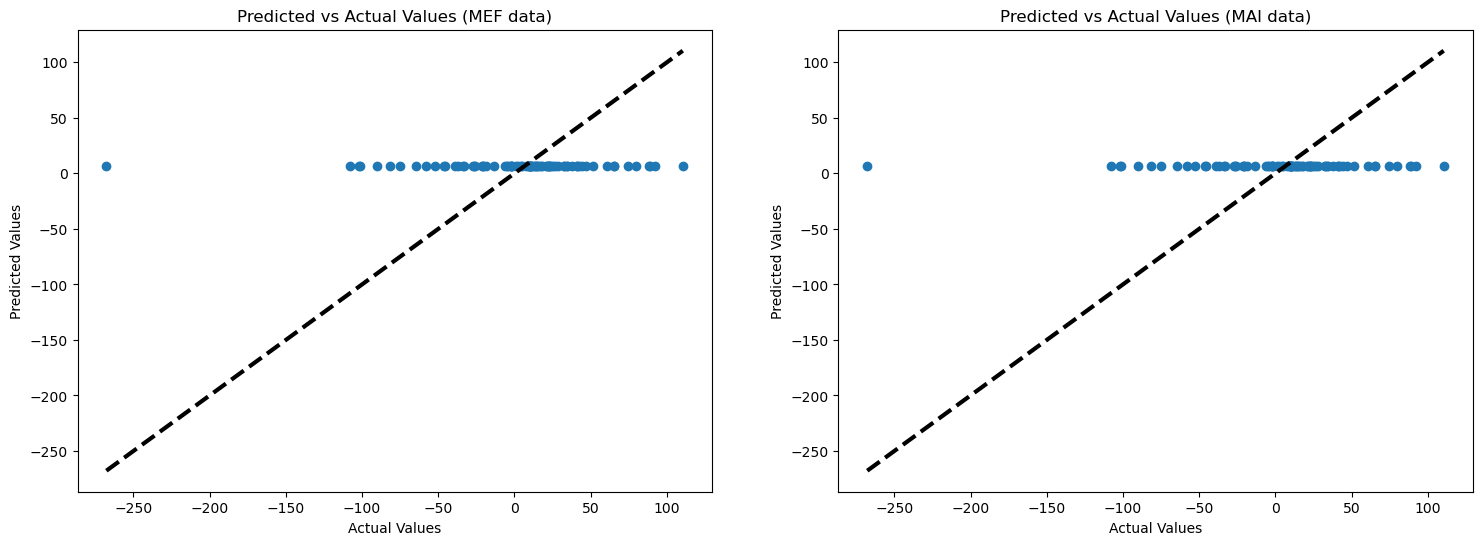
\includegraphics[width=\linewidth]{true_vs_pred_M_Regr.png}
    \caption{True vs Predicted values for monthly data (Regression)}
\end{figure}

\begin{figure}[h]
    \centering
    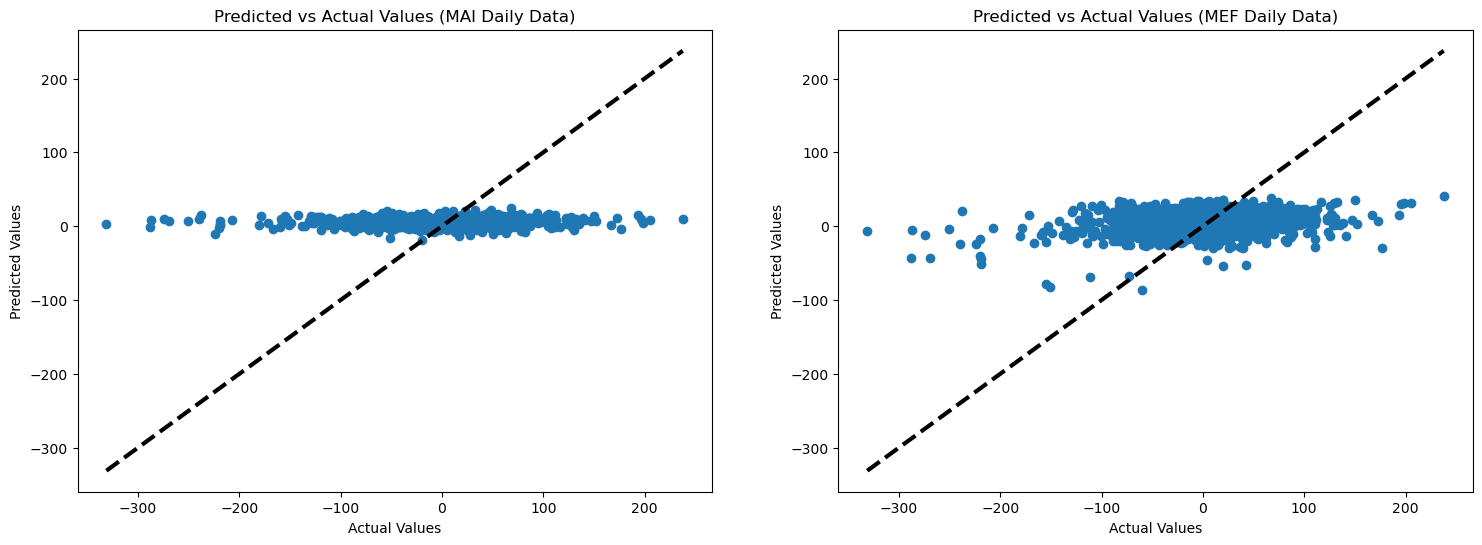
\includegraphics[width=\linewidth]{true_vs_pred_D_Regr.png}
    \caption{True vs Predicted values for daily data (Regression)}
\end{figure}


\begin{figure}[H]
    \centering 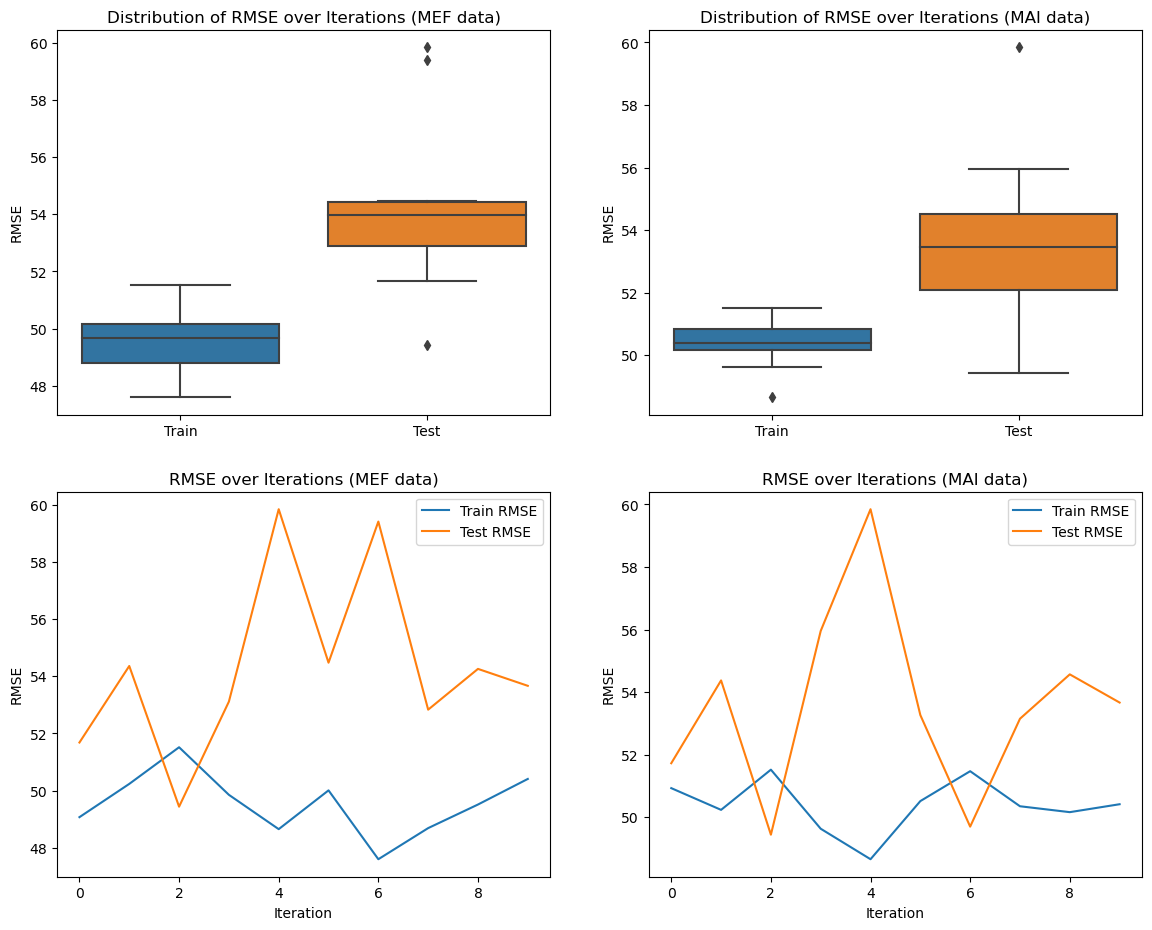
\includegraphics[width=1\linewidth]{Distribution of RMSE_Linear_M.png}
    \caption{Distribution and boxplots of RMSE over iterations, Ridge models on monthly data.}
\end{figure}

\subsubsection{Neural Network Model Results}
Even though as an initial interpretation, someone could attribute the poor performance of the regression model to its inability to capture strongly non-linear relationships, we notice that the performance of the neural network models is equally bad.
\\
We notice again the same problem, where all the predictions seem to gather close to 0, unable to follow the rough movements of the true stock returns.

\begin{figure}[H]
  \centering
  \begin{subfigure}{0.45\linewidth}
    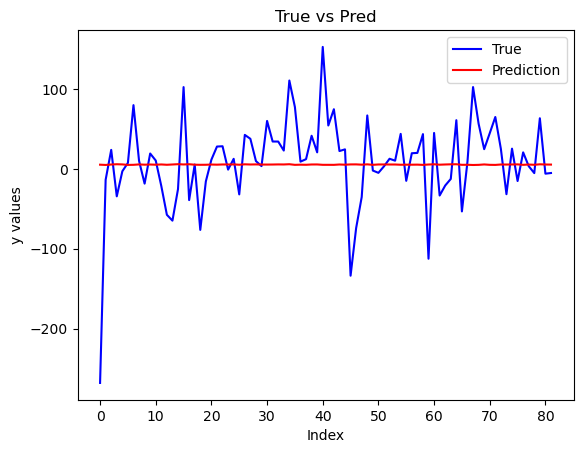
\includegraphics[width=\linewidth]{true_vs_pred_mef_M_NN.png}
    \caption{MEF monthly}
  \end{subfigure}
  \hfill
  \begin{subfigure}{0.45\linewidth}
    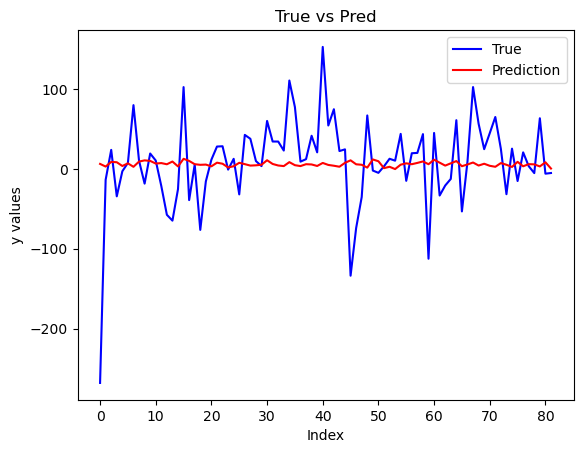
\includegraphics[width=\linewidth]{true_vs_pred_mai_M_NN.png}
    \caption{MAI monthly}
  \end{subfigure}
  \caption{True vs Predicted values for monthly data (Neural Network)}

  \end{figure}

  \begin{figure}[H]
  \centering
  \begin{subfigure}{0.45\linewidth}
    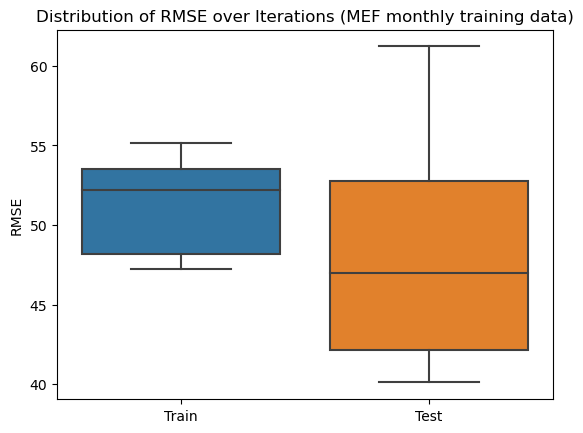
\includegraphics[width=\linewidth]{RMSE_distribution_mef_NN.png}
    \caption{MEF monthly}
  \end{subfigure}
  \hfill
  \begin{subfigure}{0.45\linewidth}
    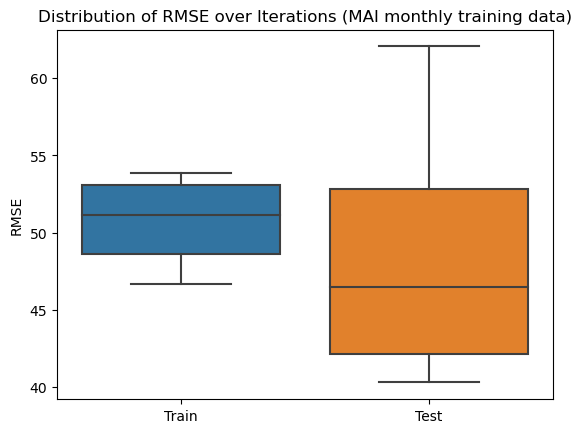
\includegraphics[width=\linewidth]{RMSE_distribution_mai_NN.png}
    \caption{MAI monthly}
  \end{subfigure}
  \caption{Distribution and boxplots of RMSE over iterations, Neural Networks on monthly data.}

  \end{figure}

  \begin{figure}[H]
  \centering
  \begin{subfigure}{0.45\linewidth}
    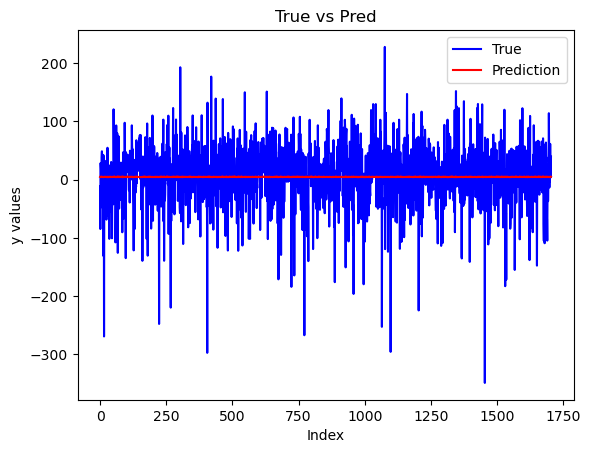
\includegraphics[width=\linewidth]{true_vs_pred_mef_D_NN.png}
    \caption{MEF daily}
  \end{subfigure}
  \hfill
  \begin{subfigure}{0.45\linewidth}
    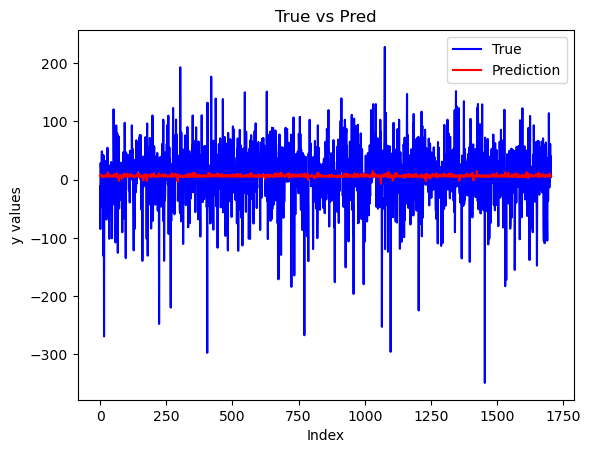
\includegraphics[width=\linewidth]{true_vs_pred_mai_D_NN.png}
    \caption{MAI daily}
  \end{subfigure}
  \caption{True vs Predicted values for daily data (Neural Network)}

  \end{figure}


\subsection{Model Selection}
The table presented in chapter 5.3.1 (Table \ref{tab:RMSE}) clearly illustrates the inefficiency of both models (Ridge Regression, Neural Network) trained with any dataset to predict the excess annualized returns of S\&P500. This cannot be interpreted as just a bad fit since all the models seem to not be trained and predicted within a very narrow range. Given these results, it wouldn't make sense to choose a model as the best performing compared to others.


\section{Discussion}

\subsection{Summary}
In this study, we endeavoured to forecast equity risk premia by employing regression and neural network models, leveraging a set of macroeconomic factors (MEF) and macroeconomic attention indices (MAI). The selection of macroeconomic factors was anchored on the seminal work by Goyal and Welch (2008), incorporating 14 features that have been previously identified as significant. Concurrently, we incorporated the eight features of macro attention indices as outlined by Fisher et al. (2022). Our target metric, the equity risk premium, was operationalized as the annualized excess return of the one-month S\&P 500 index over the short-term Treasury Bill yield.

Our research utilized data spanning from 1985 to 2018, a period for which comprehensive data was available, drawing from datasets curated in various GitHub repositories and Yahoo Finance. 

The results of our predictive modelling efforts presented a noticeable divergence from established research, showcasing significant prediction errors, indicating that the models were unable to capture the complexity of the financial data adequately.

\subsection{Interpretation of results}

The complete lack of predictive efficacy of the macro attention indices contradicts the findings in the limited relevant literature [7]. This doesn't necessarily indicate the lack of information for the stock returns these features carry. This can be supported by the fact that even the traditionally used macroeconomic factors, seem to not provide any useful predictions according to our analysis. Thus it could be reasonable that the results are a consequence of insufficient data preprocessing, lack of model complexity, or inability to capture the relationship of the features with the target variable in such a wide time frame of data. To sum up, potential reasons for the poor performance of the models include among others:

\begin{itemize}
    \item The features used may not have a strong relationship with the target variable.
    \item  Inadequate data preprocessing, such as not handling missing values correctly, or not addressing outliers.
    \item Inappropriate hyperparameter tuning.
    \item Insufficient model complexity, especially for the neural network where there are a lot of possibilities for alternative architectures.
    \item Non-stationarity of the statistical properties of the stock returns.
\end{itemize}

\subsection{Recommendations for Future Research}

Aligning with pitfalls our analysis indicated, further steps for researching the predictive power of macro attention indices can be:
\begin{itemize}
    \item Experiment with combinations of MAI and MEF features as input to the predictive models.
    \item Explore advanced preprocessing techniques, outlier detection methods, and ways to handle missing data to improve model inputs.
    \item Conduct a more extensive hyperparameter search.
    \item Explore more sophisticated modelling approaches.
    \item Focus on shorter time ranges and not on the whole dataset or perform more advanced time series analysis techniques to address non-stationarity.
\end{itemize}

\section{References}

\patchcmd{\thebibliography}{\section*{\refname}}{}{}{}

\begin{thebibliography}{9}
\bibitem{Fama1988}
\href{https://www.sciencedirect.com/science/article/pii/0304405X88900207}{Fama and French (1988). \emph{Dividend Yields and Expected Stock Returns}.}

\bibitem{Goyal2003}
\href{https://www.jstor.org/stable/4133989}{Goyal and Welch (2003). \emph{Predicting the Equity Premium with Dividend Ratios}.}

\bibitem{Lo2021}
\href{https://www.tandfonline.com/doi/full/10.1080/14697688.2023.2203844}{Lo and Singh (2003). \emph{Deep-learning models for forecasting financial risk premia and their interpretations}.}

\bibitem{Gu2019}
\href{https://dachxiu.chicagobooth.edu/download/ML.pdf}{Gu, Kelly, and Xiu (2019). \emph{Empirical Asset Pricing via Machine Learning}.}

\bibitem{Andrei2012}
\href{https://www.epfl.ch/labs/cfi/wp-content/uploads/2018/08/WP757_A2.pdf}{Andrei and Hasler (2012). \emph{Investors’ Attention and Stock Market Volatility}.}

\bibitem{Nikkinen}
\href{https://www.sciencedirect.com/science/article/pii/S104402830600024X}{Nikkinen, Omran, Sahlström, and Äijö (2006). \emph{Global stock market reactions to scheduled U.S. macroeconomic news announcements}.}

\bibitem{Ma2022}
\href{https://doi.org/10.1016/j.intfin.2022.101603}{Ma, Lu, Liu, and Huang (2022). \emph{Macroeconomic attention and stock market return predictability}.}

\end{thebibliography}

\end{document}
